\documentclass[12pt]{article}
%\usepackage{snapshot}  % Creates .dep file showing dependencies
\usepackage[a4paper, margin=0.5in]{geometry}

\usepackage{anyfontsize}
\usepackage{xcolor}
\usepackage{graphicx}
\usepackage{setspace}
\usepackage{hyperref}
\usepackage[backend=biber]{biblatex}
\usepackage{float}
\usepackage{siunitx}
\usepackage{svg}
\usepackage{xepersian}
\usepackage{algorithm2e}
\usepackage{caption}
\usepackage{amssymb}
\usepackage{amsmath}
\usepackage{enumitem}
\usepackage{bigints}
\hypersetup{colorlinks,urlcolor=blue}
%\settextfont[Scale=1.1]{Far.Mitra}

\settextfont[Scale=1.0, Size=14pt]{B Nazanin}
\defpersianfont\persiantitlefont[Scale=1.0, Size=18pt]{B Titr}
\setlatintextfont[Scale=1.0, Size=12pt]{Times New Roman}
\deflatinfont\englishtitlefont[Scale=1.0, Size=16pt]{Times New Roman Bold}

\usepackage[backend=biber]{biblatex}
\addbibresource{references.bib}


\def\labelitemi{$\diamond$}
\def\labelitemii{$\ast$}
\setcounter{secnumdepth}{0}  % Depth 0 = no section numbering

\begin{document}
	\linespread{3}
	\setstretch{1.5}
	
	% --- HEADER ROW ---
	\begin{minipage}[t]{0.7\textwidth}
		\huge\textcolor{teal!70!black}{\title\textbf{{استنباط آماری}}}
	\end{minipage}
	\hfil
	\begin{minipage}[t]{0.15\textwidth}
		\centering
		
\includegraphics[width=0.9\linewidth]{pics/logo.png}\\[6pt]
		{\small پاییز ۱۴۰۴}
	\end{minipage}
	
	
	
	{
		
		\Large{تمرین سوم}
		
		\large مرتضی ملکی‌نژاد شوشتری - ۸۱۰۱۰۴۲۵۶
		
		
	}
	
	\vspace{1.2cm}
	
	
	
	\vspace{0.3cm}
	\hrule
	\vspace{0.6cm}
%	\tableofcontents
	\section*{سوال ۱}
\lr{\subsection{a}}
ممان اول برابر میانگین و ممان دوم برابر است با 
$E(X^2) = E(X)^2 + Var(X)$
در توزیع گاما داریم:
\begin{latin}
	~\\
	$
	X \sim Gamma(\alpha, \beta) \Rightarrow E(X) = \alpha \beta \quad Var(X) = \alpha \beta^2
	\\
	\Rightarrow \hat{\beta} = \cfrac{S^2}{\bar{T}} \quad \hat{\alpha} = \cfrac{\bar{T^2}}{S^2}
	$
\end{latin}
\lr{\subsection{b}}
طبق قانون اعداد بزرگ با زیاد شدن 
\lr{n}
میانگین نمونه به سمت میانگین جامعه می‌رود. همچنین می‌توان گفت:
\begin{latin}
	$
	LLN \rightarrow E(X^2) = \mu_{population}^2 + \sigma_{population}^2 \Rightarrow 
	\sigma_{population}^2  =  E(X^2) - \mu_{population}^2
	$
\end{latin}
یعنی با زیاد شدن 
\lr{n}
واریانس نمونه نیز به واریانس جامعه نزدیک می‌شود.
پس اگر سایز نمونه زیاد باشد، عملا 
$\bar{T}$
برابر با میانگین جامعه و 
$S^2$
برابر با واریانس جامعه است پس داریم:
\begin{latin}
	$
	E(\hat{\beta})  \stackrel{n\rightarrow\infty}{=} \cfrac{\sigma^2}{\mu} = \beta
	$
\end{latin}
	یعنی 
	$\hat{\beta}$
	یک 
	\lr{estimator}
	بدون بایاس است.
	\lr{\subsection{c}}
	چون مقدار
	$\alpha$
	مشخص است، می‌توان تنها از ممان اول استفاده کرد که برابر است با 
	$\alpha \beta $
	پس یعنی 
	$\beta$
	برابر است با:
	$\cfrac{\bar{T}}{3}$
	\lr{\subsection{d}}
	با جایگذاری در فرمول‌های بخش اول داریم:
	\begin{latin}
		$
		\hat{\beta} = \cfrac{S^2}{\bar{T}} = \cfrac{10.8}{7.2} = 1.5
		\\
		\hat{\alpha} = \cfrac{\bar{T}^2}{S^2} = \cfrac{7.2^2}{10.8} = 4.8
		$
	\end{latin}
	میانگین توزیع گاما برابر است با:
	\begin{latin}
	$
	\hat{\mu}=  \hat{\alpha} \hat{\beta} = 77.76
	$
		\end{latin}
\section{سوال ۲}
\lr{\subsection{a}}
داریم:
\begin{latin}
	$
	L(\lambda) = \prod\limits_{i = 1}^n \lambda e^{-\lambda T_i} = \lambda^n e^{-\lambda (\sum_{i=0}^n T_i)}
	\Rightarrow
	l(\lambda) = n ln \lambda - \lambda \sum\limits_{i = 1}^n T_i
	$
\end{latin}
معنی 
$L(\lambda)$
این است که اگر مقدار 
$\lambda$
جامعه برابر این مقدار باشد، چه قدر احتمال  (یا چگالی احتمال) دارد که داده‌های 
$T_i$
مشاهده شوند.
\lr{\subsection{b}}
باید مقداری را پیدا کرد که  
\lr{L}
یا 
\lr{l}
در آن بیشینه می‌شوند. (چون لگاریتم صعودی است هر دو مقدار یکی است.)
با مشتق گرفتن از 
\lr{Log Likelihood}
نسبت به $\lambda$ و صفر قرار دادن آن داریم:
\begin{latin}
	$
	\cfrac{n}{\lambda} = \sum\limits_{i = 1}^n T_i  \Rightarrow \lambda = \cfrac{n}{\sum\limits_{i = 1}^n T_i } = \cfrac{1}{\bar{T}}
	$
\end{latin}
همچنین مشتق دوم این تابع برابر است با 
$\cfrac{-n}{\lambda^2}$
که همواره منفی است. این به این معنی است که اکسترممی که یافت شد درواقع ماکسیمم است.
\lr{\subsection{c}}
\begin{latin}
	$
	U = l' = \cfrac{n}{\lambda} - \sum\limits_{i = 1}^n T_i \xrightarrow{\lambda = \cfrac{1}{\bar{T}}} 
	U =  n \bar{T} - n \bar{T} = 0
	$
\end{latin}
یعنی به ازای 
$\lambda$
جامعه مقدار 
\lr{score}
صفر می‌شود.

علامت 
\lr{score}
جهت حرکت برای بیشتر کردن 
\lr{likelihood}
و مقدار آن میزان شیب را نشان می‌دهد.
\lr{\subsection{d}}
\begin{enumerate}
	\item 
	چون توزیع نمایی تنها یک متفیر دارد، عملا باید مشتق دوم 
	\lr{log likelihood}
	را حساب کرد که در قسمت قبل حساب شد و برابر است با:
	$
	\cfrac{-n}{\lambda^2}
	$
	که یعنی 
	\lr{fisher information }
	برابر است با:
	\begin{latin}
		$
		I = -E(\cfrac{\partial^2 l }{\partial \lambda^2}) = \cfrac{n}{\lambda^2}
		$
	\end{latin}
	\item 
	باید واریانس تابع 
	\lr{score}
	را حساب کرد. تابع 
	\lr{score}
	برابر است با:
	\begin{latin}
		$
		U = \cfrac{n}{\lambda} - \sum\limits_{i = 1}^n T_i 
		\xrightarrow{T_i\ are\ iid}
		E(U) = E(\cfrac{n}{\lambda}) - nE(x) = \cfrac{n}{\lambda} - \cfrac{n}{\lambda} = 0
		\\
		E(U^2) = E(\cfrac{n^2}{\lambda^2}) + E(\sum\limits_{i = 1}^n T_i)^2 - 2E(\cfrac{n}{\lambda}(\sum\limits_{i = 1}^n T_i)) 
		\Rightarrow
		 E(U^2) = \cfrac{n^2}{\lambda^2} - \cfrac{2n^2}{\lambda^2} + E((\sum\limits_{i = 1}^n T_i)^2) 
	\\
		 \xrightarrow{T_i\ are\ iid}
		 E(U^2) = (nE(X^2) + \cfrac{n(n - 1)}{2} E(X^2)) - \cfrac{n^2}{\lambda^2} 
		 = \cfrac{n(n + 1)}{2} (E(X) + Var(X)) -\cfrac{n^2}{\lambda^2} 
		 \\
		 = \cfrac{n(n + 1)}{2} * \cfrac{2}{\lambda^2} - \cfrac{n^2}{\lambda^2}
		 = \cfrac{n^2 + n}{\lambda^2} - \cfrac{n^2}{\lambda^2}
		 = \cfrac{n}{\lambda^2}
 		$
	\end{latin}
\end{enumerate}
مقدار بدست آمده از هر دو روش برابر است. 
\lr{fisher information }
درواقع میزان اطمینانی که با آن از روی یک نمونه می‌توان راجع به پارامتر جامعه صحبت کرد را نشان می‌دهد. 
\lr{fisher information}
پایین یعنی با اطمینان کمی می‌توان از روی نمونه پارامتر جامعه را بدست آورد و 
\lr{fisher information}
بالا به این معنی است که با اطمینان خوبی می‌توان از نمونه پارامتر جامعه را حدس زد.

در این مثال بدیهی است که با زیاد شدن 
\lr{n}
اطمینان در مورد پارامتر بیشتر است. همچنین اگر 
$\lambda$
مقداری زیاد داشته باشد 
\lr{fisher information }
کم می‌شود زیرا احتمال نزدیک بودن مقادیر نمونه‌ها به هم بیشتر می‌شود و نمی‌توان به خوبی 
$\lambda$
را تخمین زد.
\lr{\subsection{e}}
\begin{enumerate}
	\item 
	اثبات 
	\lr{unbias}:
	
	از قسمت 
	\lr{b}
	داریم که 
	$\lambda_{mle} = \cfrac{1}{\bar{T}}
	$
	اگر امید این متغیر را حساب کنیم داریم:
	\begin{latin}
		$
		\text{LLN} \rightarrow lim _{n \rightarrow \infty } \bar{X} = E(X)  \Rightarrow \cfrac{1}{\bar{X}} = \cfrac{1}{E(X) } \Rightarrow
		\lambda_{mle} = \cfrac{1}{\bar{X}} = \cfrac{1}{E(X)} = \lambda \Rightarrow \lambda_{mle} = \lambda
		$
	\end{latin}
	که به این معنی است که 
	$\lambda_{mle}$
	یک تخمینگر بدون بایاس است.
	\item 
	اثبات 
	\lr{consistency}:
	
	باید ثابت کرد که 
	
	\begin{latin}
		$
	(n \rightarrow\infty) \Rightarrow	P(|\cfrac{1}{\bar{X}} - \lambda| > \delta) = 0  \Rightarrow P(|\cfrac{1 - \lambda \bar{X}}{\bar{X}} > \delta) = 0
	\xrightarrow{lln} P(\cfrac{1 - \cfrac{\lambda}{\lambda}}{\bar{X}} > \delta) = 0 \Rightarrow P(0 > \delta) = 0
		$
	\end{latin}
	همه مراحل برگشت پذیر هستند. پس 
	$\lambda_{mle}$
	در احتمال همگراست و 
	\lr{consistent}
	می‌باشد.
	
	
	\item 
	اثبات حد 
	\lr{Crammer Rao}:
	
	حل نشده.
	
\end{enumerate}
\lr{\subsection{f}}
باید ممان اول با توجه به 
$\lambda$
حساب شود که برابر است با 
$\cfrac{1}{\lambda}$
پس می‌توان گفت:

\begin{latin}
	$
	E(X) = \cfrac{1}{\lambda} \Rightarrow \lambda = \cfrac{1}{E(X)} = \cfrac{1}{\bar{X}}
	$
\end{latin}
که در این جا برابر با همان تخمین 
\lr{MLE}
است. البته این لزوما در همه توزیع‌ها برقرار نیست.

\lr{\subsection{g}}
\begin{enumerate}
	\item 
	\begin{latin}
		$
		E(T) = 4.5 \Rightarrow \hat{\lambda} = \cfrac{1}{4,5}  \approx 0.22
		$
	\end{latin}
	\item 
		تخمین امید جامعه برابر با امید نمونه است. پس یعنی باید امید نمونه را حساب کرد. داریم:
	\begin{latin}
		$
		E_mle(X) = 4.5
		$
	\end{latin}
	\item 
	طبق قضیه حد مرکزی، نسبت میانگین نمونه‌ها از توزیع نرمال پیروی می‌کند. پس داریم:
	\begin{latin}
		$
		\bar{X} \sim Normal(\mu, \sigma) \Rightarrow P(\lambda \in [\bar{x} - \cfrac{\sigma}{\sqrt{n}} Z_{0.025},  \bar{x} + \cfrac{\sigma}{\sqrt{n}} Z_{0.025}]) = 0.95
		$
	\end{latin}
	چون در اینجا 
	$\sigma$
	را نداریم (
	$\sigma$ خود برابر $\lambda$ است که به دنبال یافتن آن هستیم.)
	باید از واریانس نمونه‌ای استفاده کرد. اگر سایز نمونه کم باشد باید از توزیع 
	\lr{T}
	استفاده کرد. در غیر اینصورت استفاده از توزیع 
	\lr{Z}
	نیز قابل قبول است.
\end{enumerate}
\section{سوال ۳}
استفاده از 
\lr{mle}
به طور کلی خطای کمتری دارد. این مورد بیشتر در واریانس نمود دارد زیرا بایاس هر دو روش بسیار کم است. در نمودارهای ویولنی می‌توان دید که در سایز داده‌های یکسان شکل توزیع 
\lr{mle}
و
\lr{mom}
یکسان است ولی 
\lr{mom}
نقاط 
\lr{outlier}
زیادی دارد که ناشی از واریانس بیشتر آن است.

همچنین می‌توان دید که در سایز داده 
\lr{100}
نسبت به 
\lr{25}
توزیع نمونه پراکندگی کمتری دارد. درواقع با توجه به جدول \lr{variance} می‌توان دید نسبت واریانس نمونه‌های \lr{25} تایی به \lr{100} تایی حدودا برابر 
\lr{4.01}
است که با این انتظار که واریانس با 
\lr{n}
رابطه مستقیم دارد منطبق است.
\begin{table}[h!]
	\centering
	\caption{مقایسه \lr{bias} بین دو روش در سایز داده‌های مختلف}
	\begin{latin}
	\label{tab:bias-comparison}
	\begin{tabular}{lcccc}
		\textbf{Method} & \textbf{10} & \textbf{25} & \textbf{100} & \textbf{200} \\
		\hline
		Method of Moments & -0.27498 & -0.08301 & -0.01326 & -0.00139 \\
		MLE & -0.21757 & -0.06965 & -0.01599 & -0.00622 \\
	\end{tabular}
		\end{latin}
\end{table}

\begin{table}[h!]
	\centering
	\caption{مقایسه \lr{variance} بین دو روش در سایز داده‌های مختلف}
	\begin{latin}
	\begin{tabular}{lrrrr}
		\textbf{Name} & \textbf{10} & \textbf{25} & \textbf{100} & \textbf{200} \\
		\hline
		Method of Moments & 0.88706 & 0.46533 & 0.11985 & 0.05501 \\
		MLE & 0.77585 & 0.34724 & 0.08642 & 0.03828 \\
	\end{tabular}
		\end{latin}
\end{table}


\begin{table}[h!]
	\centering
	\caption{مقایسه \lr{mse} بین دو روش در سایز داده‌های مختلف}
	\begin{latin}
	\label{tab:mse-comparison}
	\begin{tabular}{lrrrr}
		\textbf{Name} & {\textbf{10}} & {\textbf{25}} & {\textbf{100}} & {\textbf{200}}  \\
		\hline 
		Method of Moments & 0.96267 & 0.47222 & 0.12003 & 0.05501 \\
		MLE & 0.82319 & 0.35209 & 0.08668 & 0.03832 \\
	\end{tabular}
		\end{latin}
\end{table}

{
	\centering
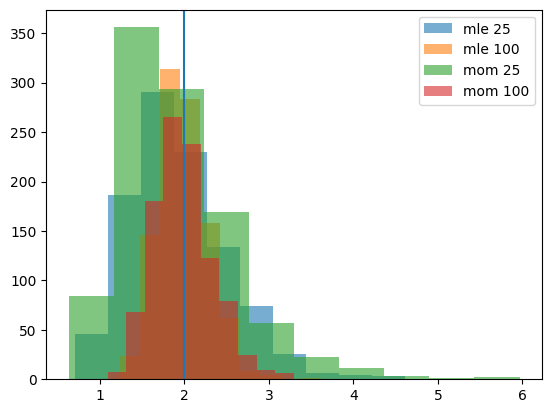
\includegraphics[width=0.8\textwidth]{pics/q3_1.png}
\captionof{figure}{هیستوگرام پارامتر مقیاس در حالت‌های مختلف}
}
{
	\centering
	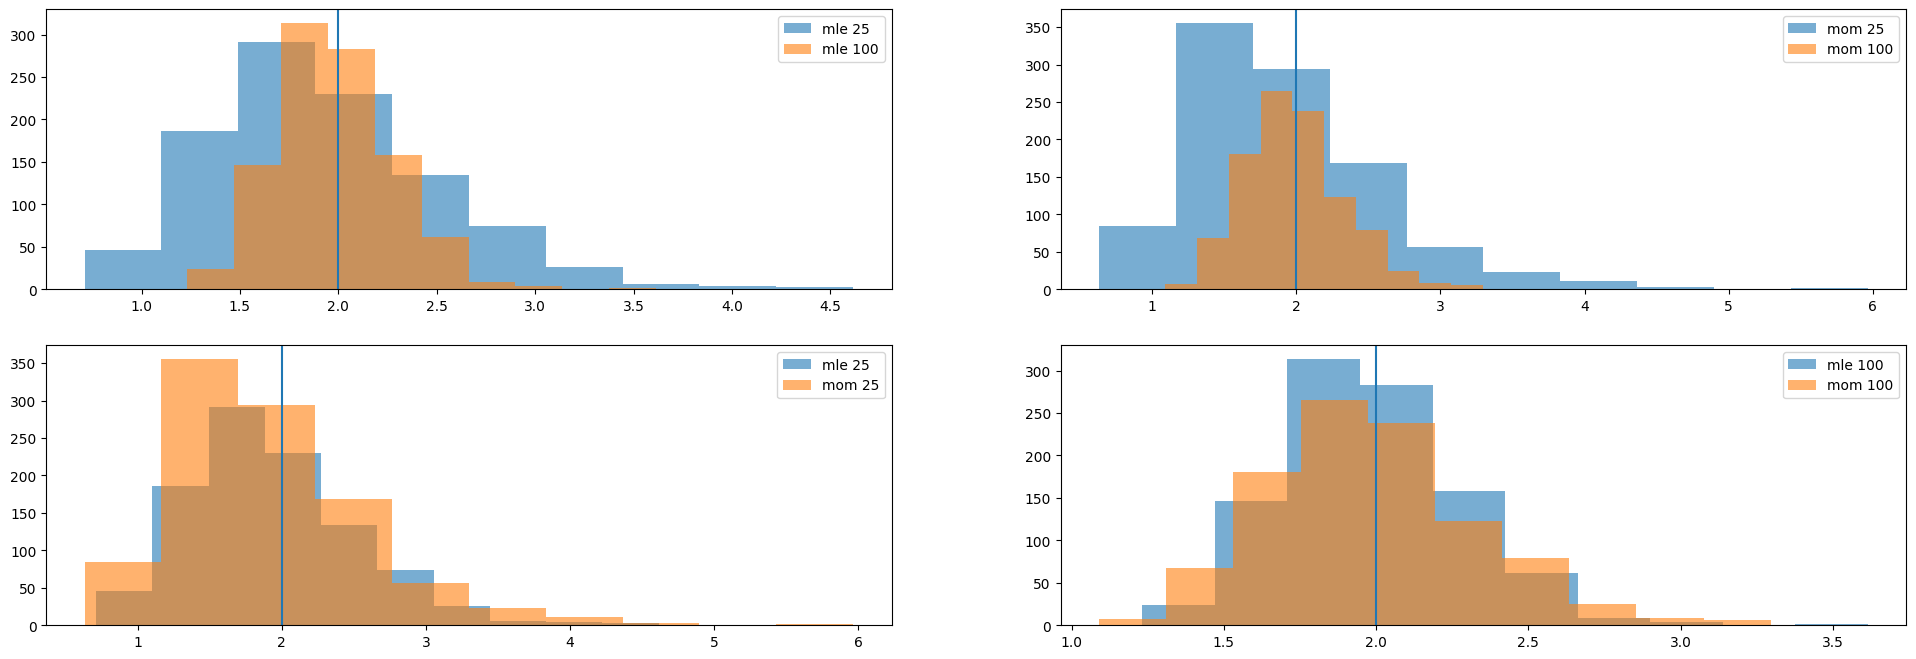
\includegraphics[width=0.8\textwidth]{pics/q3_2.png}
	\captionof{figure}{مقایسه دو به دو هیستوگرام‌های پارامتر مقیاس}
	
}
{
	\centering
	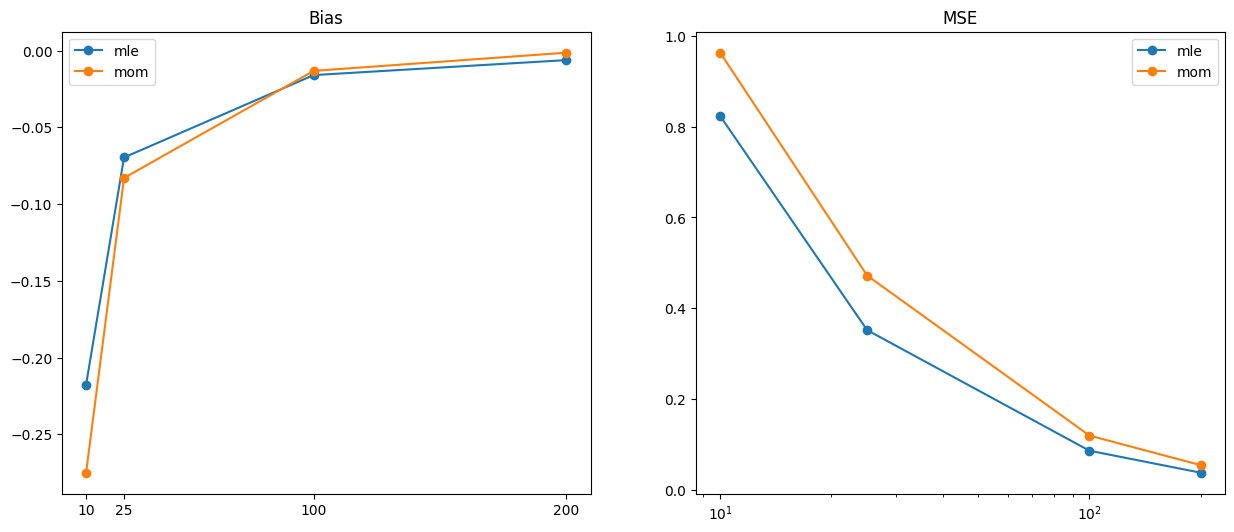
\includegraphics[width=0.8\textwidth]{pics/q3_3.png}
	\captionof{figure}{میزان خطا و بایاس به‌ازای دو روش باتوجه به سایز نمونه}
	
}
{
	\centering
	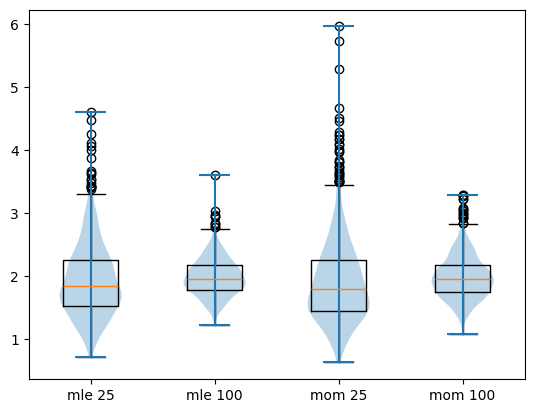
\includegraphics[width=0.8\textwidth]{pics/q3_4.png}
	\captionof{figure}{نمودار جعبه‌ای و ویالنی پارامتر مقیاس}
	
}

\section{سوال ۴}
\lr{\subsection{a}}
چون تنها داده موجود یک نمونه‌گیری است، بهترین تخمین (از دید \lr{MSE}) برای میانگین جامعه برابر میانگین نمونه است و برای واریانس جامعه مقدار 
\lr{unbias}
شده واریانس نمونه است
. یعنی داریم:
\begin{latin}
	$
	\hat{\mu} = \bar{X} = 28.4
	\\
	\hat{\sigma} = \cfrac{n}{n - 1} S^2 = \cfrac{36}{35} * 49  = 50.4
	$
\end{latin}
در 
\lr{point estimation}
هدف بیان یک عدد است که باتوجه به داده‌های موجود بهترین توصیف را از مقدار واقعی پارامتر داشته باشد. درواقع مقدار
$
E((x - \hat{x})^2)
$
کمینه شود. اما در 
\lr{interval estimation}
هدف یافتن بازه‌ای می‌باشد که با احتمال بالایی شامل پارامتر باشد. یعنی مقدار 
$
P(a < x < b)
$
بزرگتر از یک مقدار خاص باشد (برای مثال 
\lr{0.95}
)
و مقدار 
$
b - a$
خیلی زیاد نشود.
\lr{\subsection{b}}
طبق \lr{CLT} می‌دانیم توزیع 
\lr{sample mean}
یک توزیع نرمال با میانگین جامعه و واریانس 
$\cfrac{\sigma^2}{n}$
است. پس
داریم:
\begin{latin}
	$
	\cfrac{\bar{x} - \mu}{\frac{\sigma}{\sqrt{n}}} \sim Z \qquad
	Z_{0.025} \approx 1.96 \quad \sigma = 7 \quad \bar{X} = 28.4 \quad n = 36
	\Rightarrow
	CI_{0.95} = [28.4 - \cfrac{7}{6} * 1.96, 28.4 + \cfrac{7}{6} * 1.96]
	\\
	\approx [26.11, 30.69]
	$
\end{latin}
\lr{\subsection{c}}
داریم:
\begin{latin}
	$
	\cfrac{(n - 1)S^2}{\sigma^2} \sum \chi^2_{n - 1}
	\Rightarrow
	CI_{\alpha} = [\cfrac{(n - 1)S^2}{\chi^2_{n - 1, \frac{1 + \alpha}{2}}}, \cfrac{(n - 1)S^2}{\chi^2_{n - 1, \frac{1 - \alpha}{2}}}]
	\approx 
	[33.15, 85.76]
	$
\end{latin}
\lr{\subsection{d}}
فرق این‌جا با قسمت 
\lr{a}
این است که بجای توزیع 
\lr{z}
باید از توزیع 
\lr{t}
با 
\lr{n - 1}
درجه آزادی استفاده کرد و بجای واریانس جامعه باید از واریانس 
\lr{unbiased}
نمونه استفاده کرد. یعنی داریم:
\begin{latin}
	$
	s_{unbiased}^2 = \cfrac{ns^2}{n - 1} 
	\qquad 
	\cfrac{\bar{x} - \mu}{\frac{s_{unbias}}{\sqrt{n}}} \sim T_{n - 1}
	\quad 
	n = 36
	\quad 
	\bar{x} = 28.4
	\quad 
	s^2_{unbias} = \cfrac{36}{35} * 49 = 50.4  \Rightarrow s_{unbiased} \approx 7.1
	\\
	\Rightarrow
	\cfrac{28.4 - \mu}{\frac{7.1}{6}} \sim T_{35}
	\Rightarrow \mu \sim 1.18 T_{35} + 28.4
	\\
	\Rightarrow
	CI_{0.95} \approx [28.4 - 1.18 T_{35, 0.025} , 28.4 + 1.18 T_{35, 0.025}]
	\approx
	[26, 30.80]
	$
\end{latin}
بانوشتن کد این قسمت (برای گرفتن مقدار دقیق‌تر) بازه زیر حساب شد که با مقدار تئوری همخوانی دارد.
\begin{latin}
	$
	CI_{0.95} = [25.9979, 30.8021]
	$
\end{latin}
\lr{\subsection{e}}
\begin{itemize}
	\item 
	اگر درباره توزیع فرضی نباشد (برای مثال در سایز نمونه‌های پایین) استفاده از روش‌های تئوری ممکن نیست (و یا خطای بالایی دارد). زیرا توزیع 
	\lr{estimator}
	توزیع مشخصی که احتمالات در آن معلوم هستند نیست. روش 
	\lr{bootstrap}
	نمونه‌را مشابه جامعه فرض می‌کند و از آن تعدادی نمونه بر می‌دارد مقدار آماره‌ها را حساب می‌کند و بازه‌ای که در آن 
	$\alpha$
	درصد آماره‌ها قرار دارند را خروجی می‌دهد.
	\item 
	\begin{latin}

		
		\begin{algorithm}[H]
			\SetAlgoLined
			\KwIn{data $= [x_1, x_2, \dots, x_n]$, $\alpha = 0.95$, $n_{\text{boot}} = 10000$}
			\KwOut{Lower and upper confidence bounds}
			\BlankLine
			$\text{bootstrap\_data} \leftarrow [\;]$\;
			\For{$i \leftarrow 1$ \KwTo $n_{\text{boot}}$}{
				$\text{sample} \leftarrow \text{random\_choice}(\text{data}, \text{size}=n, \text{replace}=\text{True})$\;
				$\text{sample\_mean} \leftarrow \text{mean}(\text{sample})$\;
				$\text{bootstrap\_data.append}(\text{sample\_mean})$\;
			}
			$\text{bootstrap\_data.sort}()$\;
			$\text{lower\_idx} \leftarrow \lfloor n_{\text{boot}} \times (1 - \alpha)/2 \rfloor$\;
			$\text{upper\_idx} \leftarrow \lfloor n_{\text{boot}} \times (1 + \alpha)/2 \rfloor$\;
			$\text{lower} \leftarrow \text{bootstrap\_data}[\text{lower\_idx}]$\;
			$\text{upper} \leftarrow \text{bootstrap\_data}[\text{upper\_idx}]$\;
			\Return $(\text{lower}, \text{upper})$\;
			\caption{Bootstrap Confidence Interval pseudo code}
			\label{alg:bootstrap}
		\end{algorithm}
	\end{latin} 
	\item 
	روش 
	\lr{bootstrap}
	فرضی برای توزیع ندارد و تقریبا در همه موارد قابل انجام است. اما نسبت به روش‌های تئوری هزینه محاسباتی بیشتری دارد. از آنجایی که فرضی ندارد، درصورتی که میانگین واقعا مقدار مشخصی داشته باشد (برای مثال در توزیع کوشی مشخصی ندارد و روش \lr{bootstrap} به مقدار خاصی \lr{converge} نمی‌کند.) احتمال اشتباه کمتری دارد. روش 
	\lr{bootstrap}
	اگر مقدار داده زیاد باشد به مقدار واقعی 
	\lr{converge}
	می‌کند و در 
	\lr{n}
	های بالا هر دو روش جواب تقریبا یکسانی می‌دهند.
\end{itemize}
	\section{سوال ۷}
	\subsection{بخش ۱}
	اگر مقدار 
	$\alpha$
	برابر صفر باشد یعنی هیچوقت فرض صفر رد نمی‌شود. در اینصورت مقدار بتا که برابر است با احتمال 
	
	قرار دارد. در اینصورت مقدار 
	$power$
	که برابر است با 
	$P(Reject H0 | H1)$
	برابر صفر می‌شود.
	\subsection{بخش ۲}
 طبق تعاریف داریم:
	\begin{latin}
		$
		significance\ level = type1\ error = P(Reject H0 | H0) = \bigintsss\limits_0^a f_0 = F_0(\alpha) - F_0(0)
		\\
		power = P(Reject H0 | H1) =  \bigintsss\limits_0^a f_1 = F_1(\alpha) - F_1(0)
		$
	\end{latin}
	پس با فرض یکنواخت بودن توزیع در اینجا داریم:
	\begin{latin}
		$
		significance\ level = \cfrac{(\alpha - 0)}{\theta_0 - 0} = \alpha
		\\
		power = \cfrac{\alpha - 0}{\theta_1 - 0} = \cfrac{\alpha}{2}
		$
	\end{latin}
	\subsection{بخش ۳}
	\begin{latin}
		$
		significance\ level = \cfrac{1 - (1 - \alpha)}{1} = \alpha 
		\\
		power = \cfrac{1 - (1 - \alpha)}{2} = \cfrac{\alpha}{2}
		$
	\end{latin}
	\subsection{بخش ۴}
	چون توزیع‌ها یکنواخت هستند، صرفا کافیست که ناحیه 
	\lr{critical region}
	عرض مشابهی داشته باشد. یعنی برای مثال درصورتی که 
	\lr{x}
	بین 
	$0.5 - -\cfrac{\alpha}{2}$
	و 
		$0.5 + \cfrac{\alpha}{2}$
		باشد تست رد شود (البته $\alpha$ باید از $0.5$ کوچکتر باشد).
		\subsection{بخش ۵}
		اگر مقدار 
		\lr{likelihood ratio}
		اکیدا صعودی (یا نزولی) باشد، ناحیه یکتایی را می‌دهد (چون معادله $lr > k$ یک خط می‌شود. ) ولی اگر اینطور نباشد (برای مثال در اینجا نیست) ممکن است نواحی مختلفی یافت شوند.
	\subsection{بخش ۶}
	در اینصورت مقدار 
	\lr{significance level}
	و 
	\lr{power}
	عوض می‌شود.
	\section{سوال ۹}
	\subsection{بخش \lr{a}}
	\subsubsection{۱}
	\begin{latin}
		$
		z = \cfrac{9.75 - 10}{\frac{0.5}{5}} = 2.5
		$
	\end{latin}
	\subsubsection{۲}
	اگر مقدار 
	\lr{critical region}
	را برای 
	\lr{two sided}
	حساب کنیم بدست می‌آید 
	\lr{H0}
	وقتی رد می‌شود که 
	$|z|$
	بزرگتر از 
	\lr{1.96}
	باشد. از آنجایی که این جا این مقدار بزرگتر است پس فرض 
	\lr{H0}
	رد می‌شود. 
	
	\subsubsection{۳}
	اگر 
	\lr{P value}
	را بخواهیم برای این نمونه بدست آوریم برابر است با:
	$2P(Z > 2.5)$
	که برابر است با
	$0.0124$
	از آنجایی که این مقدار از 
	$0.05$
	کمتر است فرض صفر رد می‌شود.
	
	\lr{P Value}
	درواقع احتمال رخ دادن داده در صورت درست بودن فرض صفر است. هرچقدر این مقدار کمتر باشد، احتمال رخ دادن داده کمتر است اگر احتمال مشاهده در تئوری کم باشد ولی در عمل زیاد باشد یعنی فرض صفر احتمالا اشتباه است. برای همین در تست‌ها به دنبال کمینه کردن \lr{p value} هستیم. در اینجا چون
	\lr{two tailed}
	است و هر دو دم را باید درنظر گرفت، این مقدار ضربدر دو می‌شود.
	
	\subsubsection{۴}
	همانطور که ذکر شد، اگر مقدار 
	\lr{p value}
	از 
	$\alpha = 0.05$
	کمتر باشد، فرض صفر رد می‌شود.
	\subsection{بخش \lr{b}}
	\subsubsection{۱}
	\begin{latin}
		$
		Z_{0.025} = 1.96 \quad \sigma = 0.5 \quad \bar{x} = 9.75
		\Rightarrow
		CI_{0.95} = [9.75 - 1.96 * \cfrac{0.5}{5}, 9.75 + 1.96 * \cfrac{0.5}{5}]
		= [9.554, 9.946]
		$
	\end{latin}

\subsubsection{۲}
چون مقدار 
$\mu_0 = 10$
در 
\lr{confidence interval}
قرار ندارد، یعنی به احتمال 
\lr{95}
درصد میانگین جامعه این مقدار نیست. که این همان مفهوم 
\lr{Hypothesis testing}
است. درواقع در بازه اطمینان هدف یافتن زیرمجموعه‌ای از توزیع است که شامل مقدار واقعی باشد، ولی در 
\lr{Hypothesis testing}
هدف یافتن زیرمجموعه‌ای از توزیع است که مقدار واقعی در آن نباشد و با قرار گرفتن داده در آن بازه نتیجه گرفت که فرض اولیه برای داده غلط است.
\subsection{۳}
%در محاسبه 
%\lr{critical region}
%این مقدار برای آماره 
%\lr{z}
%بدست آمد. اگر این مقدار را برای خود میانگین حساب کنیم داریم: 
%\begin{latin}
%	$
%	|z| > 1.96 \Rightarrow 10 |\bar{X} - \mu| > 1.96 \Rightarrow |9.75 - \mu| > 0.196 \Rightarrow \mu > 9.946\ or\ \mu < 9.554
%	\\
%		|z| > 1.96 \Rightarrow 10 |\bar{X} - \mu| > 1.96 \Rightarrow |10  - \bar{x}| > 0.196 \Rightarrow \bar{x} < 9.804\ or\ \bar{x} > 10.196
%	$
%\end{latin}
باتوجه به اینکه بازه محاسبه شده شامل مقدار 
\lr{10}
نیست یعنی به احتمال 
\lr{95}
درصد میانگین برابر مقدار 
\lr{10}
نیست.
\subsection{۴}
در تست 
\lr{two sided}
این دو درواقع یکی هستند. یعنی اگر مقدار $\mu_0$ در 
\lr{confidence interval}
با 
\lr{confidence level}
برابر با 
$1 - \alpha$
نباشد،‌ تست آن با 
\lr{significance level}
برابر با 
$\alpha$
رد می‌شود.

	\section{سوال ۱۲}
	\lr{\subsection{a}}
	\subsubsection{۱}
	\begin{latin}
		$
		LR 
		= \cfrac{L(\theta_1)}{L(\theta_0)}
		= \cfrac{\theta_1 e^{-\theta_1 x}}{\theta_0 e^ {-\theta_0 x}}
		= \cfrac{\theta_1}{\theta_0} * e^{-(\theta_1 - \theta_0) x }
		= \cfrac{\theta_1}{\theta_0} * e^{(\theta_0 - \theta_1) x}
		$
	\end{latin}
	برای چندین ورودی 
	\lr{LR}
	ها در هم ضرب می‌شوند پس داریم:
	\begin{latin}
		$
		LR = (\cfrac{\theta_1}{\theta_0})^n  e^{-(\theta_0 - \theta_1) \sum\limits_{i = 1}^n X_i }
		$
	\end{latin}
	\subsubsection{۲}
	داریم:
	\begin{latin}
		$
		P(X < x  | H0) < \alpha 
		\Rightarrow
		1 - e^{-\lambda x} < \alpha \Rightarrow e^{-\lambda x} > 1 - \alpha
		$

	\end{latin}
			پس یعنی 
	$
	T(x)
	= 
	e ^{-\lambda x}
	$
	\lr{\subsection{b}}
	\subsubsection{۱}
	در 
	\lr{Hypothesis Testing}
	تست براساس 
	\lr{likelihood ratio}
	قوی‌ترین 
	\lr{power}
	را دارد.
	\subsubsection{۲}
	براساس لم نیمن پیرسون باید تست 
	\lr{likelihood ratio}
	را بنویسیم. باتوجه به اینکه تخمین 
	\lr{mle}
	پارامتر برابر با 
	$\cfrac{1}{\bar{x}}$
	است می‌توان تست را نوشت. البته قبل از آن باید چک کرد که این مقدار از 
	$\theta_0$
	بزرگ‌تر باشد زیرا اگر کوچک‌تر باشد، دیگر 
	$sup L(\theta_1)$
	برابر 
	\lr{mle}
	نمی‌شود و فرض صفر رد نمی‌شود. (این محاسبات از سوال ۱۳ کپی شده‌اند.)
	\begin{latin}
		$
		\Lambda = \cfrac{L_0}{L_{mle}} = (\bar{x} \theta_0)^n e^{n(1 -\theta_0 n \bar{x})}
		\Rightarrow -2log \Lambda = -2 (n log (\bar{X \theta_0}) + n(1 - \theta_0 n \bar{X})) = 2n (\bar{X} \theta_0 -1-log (\bar{X} \theta_0))
		\xrightarrow{Y = \bar{X} \theta_0} -2 log \Lambda = 2n (y - 1 - log y)
		$
	\end{latin}
	باید مقادیر زیاد عبارت داخل پرانتز را یافت. همچنین با توجه به اینکه فرض 
	\lr{H1}
	برای میانگین بزرگتر است می‌توان انتظار داشت که:
	\begin{latin}
		$
		\theta_1 > \theta_0 \Rightarrow \cfrac{1}{\theta_1} < \cfrac{1}{\theta_0} \Rightarrow \cfrac{\theta_0}{\theta_1} < 1 \Rightarrow \theta_0 \bar{x} < 1
		$
	\end{latin}
	{
		\centering
		\label{q12_shape}
		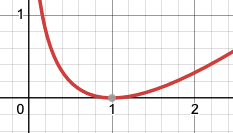
\includegraphics[width=0.8\textwidth] {pics/q12_1.png}
		\captionof{figure}{شکل تابع $y - 1 - log(y)$}
	}
با توجه به شکل 
\ref{q12_shape}
و این که
\lr{y}
کوچکتر از یک است، پس می‌توان گفت هدف یافتن مقادیر کم 
\lr{y}
است یعنی اگر 
$\theta_0 \bar{x}$
از مقداری کوچکتر باشد تست رد می‌شود. که این مقدار باتوجه به 
\lr{significance level}
بدست می‌آید. بطور دقیق‌تر داریم:
\begin{latin}
	$
	CR = \theta_0 \bar{X} < c \Rightarrow CI = \bar{X} < \cfrac{c}{\theta_0}
	$
\end{latin}

	
	\subsubsection{۳}
باتوجه به قسمت قبل باید مقدار 
\lr{c}
را طوری تعیین کرد که نامساوی درست دربیاید. پس داریم:
\begin{latin}
$
P_0(\bar{X} < \cfrac{c}{\theta_0}) = \alpha \Rightarrow 1 - e^{-\theta0 x } = \alpha \Rightarrow x = \cfrac{-ln (\alpha - 1)}{\theta_0}
$
\end{latin}
\subsubsection{۴}
\begin{latin}

$
P_1 (X > \cfrac{-ln (\alpha - 1)}{\theta_0})  = e^{-\theta_1 \cfrac{-ln (\alpha - 1)}{\theta_0}} 
= e^{\theta_1 \cfrac{ln (\alpha - 1)}{\theta_0}}  
= e^{\cfrac{\theta_1}{\theta_0}} * (\alpha - 1)
$
\end{latin}
	\lr{\subsection{c}}
	\lr{\subsection{d}}
	\lr{\subsection{e}}
	\subsubsection{۱}
	در تست فرضیه هدف چک کردن درستی 
	\lr{H0}
	می‌باشد. پس به دنبال این هستیم که با یک احتمال ثابت (برای مثال ۹۵ درصد) دید فرض صفر درست است یا خیر. هدف چک کردن درستی 
	\lr{H1}
	نیست، همچنین اصل بر این است که فرض صفر درست است و برای اثبات خلاف این باید تلاش شود. برای همین فرض صفر و فرض جایگزین عملا دو نقش متفاوت دارند.
\subsubsection{۲}
زیرا احتمال رخداد به شرط فرض صفر بررسی می‌شود. اگر برای مثال با تستی به سایز 
$0.05$
فرض صفر رد شود، یعنی به احتمال ۹۵ درصد فرض صفر اشتباه است اما راجع به فرض دیگر هیچ حرفی زده نمی‌شود. حتی اگر مقدار \lr{power} را نیز دخیل کرد. ممکن است خطای نوع ۲ بالا باشد.
	
	\section{سوال ۱۳}
	\subsection{۱}
	\begin{latin}
		$
		L = \theta^n e^{-\theta \sum\limits_{i = 1}^n x_i}  = \theta^n e^{-\theta n\bar{x}}   
		\Rightarrow
		\cfrac{\partial L}{\partial \theta} = n \theta^{n - 1} e^{-\theta n \bar{x}} - n \bar{x} \theta^n e^{-\theta n \bar{x}}  
		= e^{-\theta n \bar{x}} \theta^{n - 1}n (1 - \bar{x} \theta) = 0
		\Rightarrow 
		\hat{\theta} = \cfrac{1}{\bar{x}}
		$
	\end{latin}
	باید مقدار 
	$\cfrac{L_0}{L_{mle}}$
	را حساب کرد:
	\begin{latin}
		$
		\Lambda = \cfrac{L(\theta_0)}{L_{mle}} = \cfrac{L(\theta_0)}{\cfrac{e^{-n}}{\bar{x}^n}} = (\bar{x} \theta_0) ^n e^{- \theta_0 n \bar{x} + n}
		 = 
		 (\bar{x} \theta_0)^n e^{n(1 - \theta_0 \bar{x} ) }
		$
	\end{latin}
	هر چه این مقدار کمتر باشد فرض صفر نامحتمل تر است.
	\subsection{۲}
	انتظار می‌رود که توزیع 
	$
	-2log \Lambda 
	$
	برابر با توزیع 
	$\chi^2$
	باشد. با محاسبه 
	$
	\Lambda 
	$  
	داریم:
	\begin{latin}
		$
		-2 log \Lambda = -2 ( n log( \bar{x}) + n log (\theta_0 )  + n (1 - \theta_0 \bar{x}) )
		= -2n (log \bar{x} \theta_0) + 1 - \theta_0 \bar{x})
		$
	\end{latin}
اگر قرار دهیم 
$y = \theta_0 \bar{x}$
داریم:
\begin{latin}
	$
	-2 log \Lambda = 2n (y - 1 - log (y))
	$
\end{latin}
که طبق 
\lr{clt}
می‌دانیم توزیعی به شکل نرمال دارد و میانگین آن برابر یک و واریانس آن برابر 
$
\cfrac{1}{\sqrt{n}}
$
می‌باشد (اگر \lr{n} به سمت بینهایت برود)
اگر 
$g(y) = 1 - y - log(y)$
داریم \cite{delta_method}:
\begin{latin}
	$
	y \sim Normal(1, \cfrac{\sigma^2 }{\sqrt{n}}) \Rightarrow 
	\sqrt{n} (y - 1) \sim Normal(0, \sigma^2)
	\\
	\xrightarrow{second\ order\ delta\ method}
	n (g(Y) - g(1)) = \cfrac{1}{2} g''(1) n (Y - 1)^2
	\Rightarrow 2n (g(Y) - g(1)) =  g''(1) (\sqrt{n} (Y - 1))^2 \xrightarrow{g''(1) = 1} -2log \Lambda = (\sqrt{n} (Y - 1))^2
	\xrightarrow{n(Y - 1) \sim Z}  -2 log \Lambda \sim Z^2 \sim \chi^2_1
	$
\end{latin}
که مطابق انتظار است.
	
	\section{سوال ۱۴}
	توزیع \lr{T} شکلی شبیه به توزیع 
	\lr{Z}
	ولی با دم‌های سنگین تر دارد. هم در جدول 
	$P(X > 2)$
	و هم در نمودار توزیع آن می‌توان این مورد را دید.
	
	در چندک‌ها نیز می‌توان نزدیک بودن 
	\lr{t}
	و
	\lr{z}
	را در مقادیر نزدیک به وسط و دور شدن آن‌ها از هم را در دم‌ها دید.
	{
	\centering
	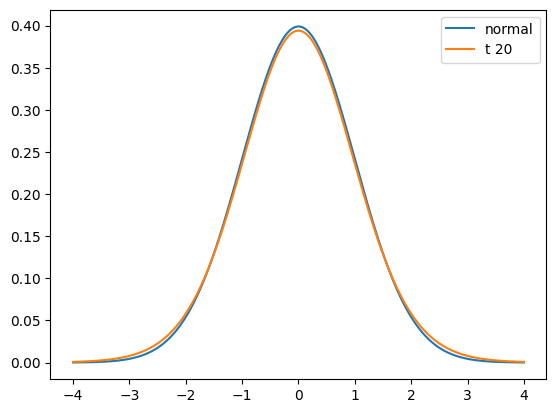
\includegraphics[width=0.8\textwidth] {pics/q14.png}
	\captionof{figure}{شکل توزیع نرمال و \lr{t} با بیست درجه آزادی}
	}
	
	\begin{table}[h]
		\centering
		\caption{
		مقدار 
		$P(X > 2)$
		در توزیع‌ها براساس \lr{CDF} و خود داده. می‌توان دید که دم توزیع \lr{T} سنگین تر است.
		}
		\begin{latin}
		\begin{tabular}{l c c}
			\textbf{Method} & \textbf{$T_{20}$ } & \textbf{Normal } \\
			Using CDF & 0.02963276772328527 & 0.02275013194817921 \\
			Using data & 0.029188273948070706 & 0.02261224040805962 \\
		\end{tabular}
				\end{latin}
	\end{table}
	

\begin{table}[h]
	\centering
					\caption{احتمال چندک‌ها می‌توان دید با زیاد شدن چندک تفاوت \lr{t} و \lr{normal} بیشتر می‌شود.}
			\begin{latin}
	\begin{tabular}{l c c}
		Quantile & \multicolumn{1}{c}{Normal} & \multicolumn{1}{c}{$t_{20}$} \\
		0.90  & 0.0023296725257150068  & 0.005049305454427419   \\
		0.95  & 0.0005953537100114529  & 0.002041047172798491   \\
		0.975 & 0.0002834035558143255  & 0.0012861077730186043  \\
	\end{tabular}
				\end{latin}
	\label{tab:tail_probs}
\end{table}

% Second table: Probability of quantile  
\begin{table}[h]
	\centering
					\caption{چندک احتمالات. تابع نرمال چندک‌های بیشتری دارد (زیرا شیب شدیدتری دارد)}
	\begin{latin}
	\begin{tabular}{l c c}
		Quantile & \multicolumn{1}{c}{Normal} & \multicolumn{1}{c}{$t_{20}$} \\
		0.90  & 0.36773640422121634 & 0.36181952769893855 \\
		0.95  & 0.39074191909301725 & 0.385498242369079   \\
		0.975 & 0.3969485720092071  & 0.39192196071191104 \\

	\end{tabular}
				\end{latin}
	\label{tab:quantiles}
\end{table}
\section{مراجع}
\begin{latin}
	\printbibliography
\end{latin}

	
\end{document}